% -*- root: ../Manual.tex -*-
\chapter{\LaTeX\ avanzado}
\label{chap:LaTeXAvanzado}

Una vez que ya nos manejamos con las cosas básicas de \LaTeX, vamos a pasar a cosas más avanzadas, como las etiquetas, índices, marcos y Tikz. También veremos parte de desarrollo de paquetes y clases de \LaTeX: cómo crear comandos y entornos y modificarlos para que hagan lo que nosotros queremos. Para eso, antes veremos cómo funciona exactamente \LaTeX, que nos ayudará a la hora de entender por qué tenemos que hacer ciertas cosas, como compilar dos veces, o qué es lo que puede estar fallando cuando algo no funciona.

\section{¿Cómo funciona \LaTeX?}
\label{sec:FuncionamientoLaTeX}

El capítulo anterior pretendía ser un tutorial básico de \LaTeX, para que podamos ponernos a escribir rápidamente. Pero para avanzar, creo que es importante saber cómo funciona este sistema, más que nada para entender de dónde salen los errores y saber exactamente qué es lo que estamos haciendo. Además, como curiosidad informática tampoco viene nada mal.

Para ser precisos, más que de \LaTeX\ deberíamos hablar de \TeX, que es el ``núcleo'' escrito por Donald Knuth. Este núcleo es un compilador que, a grandes rasgos, tiene dos fases: la de expansión y la de compilación.

Cuando compilamos un documento para generar un PDF, lo que va haciendo \TeX\ es ir leyéndolo carácter a carácter, e ir traduciéndolo. Los caracteres normales se pasan sin modificar, y los comandos (los que empiezan por \textbackslash, como \verb|\textbf|) se expanden.

La expansión de un comando no es más que sustituirlo por su definición sustituyendo los argumentos. Por ejemplo, yo puedo definir el comando \verb|\vector|, que recibe un argumento (denotado por \verb|#1|) y que se expande como \verb|$\mathbf{#1}$|. Así, cuando \TeX\ encuentre \verb|\vector{a}| lo sustituirá por \verb|$\mathbf{a}$|. Este proceso se va realizando de forma recursiva: cuando el compilador expande un comando y se encuentra que la expansión ha metido más comandos, los expande a ellos también. Todo esto se hace en orden de izquierda a derecha.

Así, comando a comando, \TeX\ va expandiendo el documento hasta llegar a la forma más básica, que son los comandos primitivos de \TeX, que simplemente dicen cosas tan de bajo nivel ``añade este carácter a la línea'' o ``ahora usa esta fuente''. Con esos comandos, \TeX\ va decidiendo cómo va a ser la estructura del PDF que va a generar (los saltos de línea o de página, o la colocación de las imágenes, por ejemplo).

Finalmente, esa información se pasa a la ``segunda etapa'' de \TeX, que transforma esos comandos primitivos en un formato estándar para un documento que nosotros podamos visualizar: normalmente es PDF, pero también pueden ser otros como DVI.

La parte específica de \LaTeX\ consiste en comandos adicionales que facilitan la vida al usuario, pero a grandes rasgos el proceso de compilación es el mismo.

En la práctica, hay algunas cosas algo más complicadas, pero básicamente así funciona \LaTeX. Lo primero que leerá del documento será el \verb|\documentclass|, que le dirá qué archivo base cargar: ese archivo cargará los comandos de \LaTeX\ básicos y prepará el documento (tipo de fuente, márgenes, papel, etc). Después, las sentencias \verb|\usepackage| cargarán otros documentos con más macros y comandos, y en cuanto empiece el documento con \verb|\begin{document}| el compilador empezará a procesar todos esos caracteres y comandos escritos, expandiendo estos últimos hasta llegar a las instrucciones primitivas para mostrar tu PDF.

\paragraph{¿Esto es importante?} Algo sí, más que nada porque nos explica de dónde salen dos tipos problemas muy habituales. El primero son los relacionados con la expansión de comandos: \LaTeX\ no es como un lenguaje de programación donde primero se evalúan los argumentos y luego se le pasan a la función. Aquí es al revés: primero se desarrolla la función (el comando) y luego se procesan los argumentos. Y si en algún momento algo no cuadra (cosa probable) la compilación falla.

La otra cuestión es algo que no hemos dicho explícitamente, pero que se puede ver: \TeX\ es un sistema de una sola pasada. Lee el fichero y va procesando según le llega, pero en ningún momento mira hacia atrás ni hacia delante\footnote{Por ejemplo, redefinir un comando a mitad del documento sólo afecta a partir de ese punto, no antes.}. El principal inconveniente es que a veces tendremos que recompilar el documento para que pille todos los datos, como las referencias. Las referencias las escribe \LaTeX\ en un documento aparte cuando se las encuentra, así que si ponemos una referencia antes de declarar la etiqueta, no va a saber resolverlo. En la segunda pasada ya se encontrará esa etiqueta declarada en el archivo aparte así que ya podrá rellenar el comando \verb|\ref| correctamente.

Para más información sobre cómo funciona \LaTeX, es recomendable echarle un ojo al libro \textit{\TeX\ for the Impatient} o \textit{The \TeX Book}.

\section{\LaTeX\ para usuarios avanzados}

A lo largo de esta sección vamos a ver algunos aspectos de \LaTeX\ que o bien nos dan más opciones para crear mejores documentos, nos facilitan la vida a la hora de escribir documentos o nos permiten personalizar ciertas partes del documento. Y todo esto usando comandos estándar y sin tener que desarrollar nada. Todavía.

La idea de la sección es ir de las partes más sencillas a las más difíciles, aunque esto siempre es subjetivo así que es recomendable echarle un ojo a todo por si acaso.

\subsection{¿Dónde están documentados los paquetes?}
\label{sec:Texdoc}

\index{texdoc}
Aunque en el mundo de la informática no suele ser lo habitual, la mayoría de los paquetes de \LaTeX\ que podamos usar están bien documentados, con documentación que es accesible desde tu ordenador. Lo más fácil es usar el comando \textit{texdoc}: si desde la terminal ejecutas \texttt{texdoc nombrepaquete} se abrirá un PDF con la documentación del paquete.

Si no, en Internet suelen estar las soluciones. Además de tener el repositorio central \href{https://www.ctan.org/?lang=en}{CTAN}, también está \href{http://tex.stackexchange.com}{TeX - Stack Exchange} para resolver dudas y, por supuesto, Google.

\subsection{Cambiando los márgenes del documento}

\index{geometry}
\index{Margen}
\LaTeX\ viene con unos márgenes determinados por defecto según la clase que usemos. Por suerte, se puede modificar fácilmente, simplemente con el paquete \textit{geometry}. La sintaxis es muy sencilla, poniendo en el preámbulo (antes del \verb|\begin{document}|) lo siguiente:

\begin{minted}{latex}
\usepackage[left=3cm, right=1cm, top=3cm, bottom=2cm]{geometry} % Márgenes
\end{minted}

Como es fácil adivinar, \textit{left, right, top, bottom} se refieren a los márgenes izquierdo, derecho, superior e inferior del documento. El paquete tiene varias opciones más, todas documentadas apropiadamente en su \textit{texdoc} (ver \fref{sec:Texdoc}), pero en general son bastante menos habituales y no hace falta que las revisemos aquí.

\subsection{Manejando documentos grandes con varios archivos}
\label{sec:ExternalFiles}

\cindex{input}
Una ventaja de \LaTeX\ es que es muy fácil manejar documentos grandes, con muchas líneas. Si vemos que mantenerlo todo en un mismo archivo se hace incómodo, podemos separarlo en varios archivos distintos e importarlos en el documento principal con el comando \verb|\input|.

\begin{minted}{latex}
\documentclass{article}

\begin{document}
Empezamos aquí con una introducción...

\input{Seccion1.tex}
\input{Seccion2.tex}

LaTeX meterá automáticamente el contenido de los archivos que le hemos dicho
 y compilará todo como un único documento.
\end{document}
\end{minted}

El comando \verb|\input| recibe como argumento el nombre del archivo a incluir. Si el archivo está en otro directorio (por ejemplo, en un subdirectorio en la misma carpeta) tendremos que poner la ruta relativa (p.e., \verb|\input{tex/Seccion1.tex}|).

\subsection{Cómo personalizar la tabla de contenidos y la numeración de secciones}
\label{sec:Contadores}

La tabla de contenidos de \LaTeX\ se genera automáticamente a partir de las secciones y subsecciones del documento. Aunque los valores por defecto suelen estar bien, a veces querremos cambiarlo. Por ejemplo, si queremos que aparezcan secciones, subsecciones y subsubsecciones en la tabla de contenidos, tendremos que poner lo siguiente en el preámbulo

\index{tocdepth}
\begin{minted}{latex}
\setcounter{tocdepth}{3}
\end{minted}

El $3$ es la profundidad máxima de la tabla (sin contar capítulos). Si quisiésemos sólo secciones, podríamos poner un $1$ en su lugar, por ejemplo.

\LaTeX\ también nos permite cambiar cómo aparecen los contadores de sección, subsección y demás. La sintaxis en general es la siguiente:

\begin{minted}{latex}
% En general:
\renewcommand{\the[contador]}{\the[otrocontador]. \forma{[contador]}}

% Ejemplo: Secciones con numeros romanos
\renewcommand{\thesection}{\Roman{section}}

% Otro mas: Subsecciones con el numero de seccion de antes
% y contador en numeros.
\renewcommand{\thesubsection}{\thesection .\arabic{subsection}}

% En realidad podemos poner lo que queramos en el segundo
% argumento:
\renewcommand{\thesubsubsection}{Esta es la subseccion \alph{subsection}}
\end{minted}

\cindex{arabic}\cindex{alph, Alph}\cindex{roman, Roman}
Podemos modificar los contadores que queramos: todos tienen el mismo nombre que el comando correspondiente (p.e., \verb|\section| tiene como contador \textit{section}). En cuanto a las formas de imprimir el número concreto, tenemos cinco posibilidades: \verb|\arabic|, que nos saca números (1,2,3, ...); \verb|\alph| o \verb|\Alph| que nos sacará letras (a,b,c) en minúsculas o mayúsuculas; y \verb|\roman| o \verb|\Roman| que nos sacarán números romanos (I, II, IV...) en minúsculas y mayúsculas respectivamente.

\subsection{Referencias todavía más automáticas: fancyref}
\label{sec:fancyref}

\index{fancyref}
\cindex{fref}
Hay un paquete adicional que mejora las características de las referencias de \LaTeX\, que se llama \textit{fancyref}\footnote{Para poder usar \textit{fancyref} en el documento, sólo hay que añadir \texttt{$\backslash$usepackage\{fancyref\}} en el preámbulo del documento. Ver la \fref{sec:EstructuraDocumento} para saber qué es exactamente el preámbulo.}. Este paquete introduce el comando \verb|\fref|, que saca la referencia con el nombre que le corresponde y con el enlace. Además, \textit{fancyref} tiene un formato ``vario'' que muestra la página en la que está lo que estemos referenciando.

\begin{LTXexample}[pos=r]
Antes usabamos \ref{eq:SuperImportante},
pero tambien podemos hablar de la
\fref{eq:SuperImportante}, de la
\fref{sec:EstructuraDocumento} o
de la \fref[vario]{sec:Tablas}.
\end{LTXexample}

\textit{fancyref} depende de que las etiquetas tengan un cierto nombre, de la forma \textit{prefijo:Identificador}, para poner el nombre correcto. Estos prefijos están en la \fref{tab:PrefjosFref}.

Adicionalmente, hemos creado el paquete \textit{fancysprefs} que traducen los prefijos de \textit{fancyref} al español y añade algunos comandos para incluir el nombre de lo que estamos referenciando automáticamente. Este paquete está descrito en la \fref{sec:fancysprefs}.

\begin{table}[hbtp]
\centering
\begin{tabular}{l|l}
\textbf{Elemento} & \textbf{Prefijo} \\ \toprule
Capítulo & chap \\
Sección & sec \\
Ecuación & eq \\
Figura & fig \\
Tabla & tab \\
Ejercicio & ej \\
Proposición & prop \\
Lema & lem \\
Teorema & thm \\
Definición & def
\end{tabular}
\caption{Prefijos establecidos para que \texttt{fref} funcione correctamente.}
\label{tab:PrefjosFref}
\end{table}

\subsection{Estilos de página: pies y cabeceras}

\index{fancyhdr}
\index{Cabeceras}
\index{Pie de página}
Podemos personalizar los estilos de página como queramos usando el paquete \textit{fancyhdr} y configurándolo en el preámbulo. Por ejemplo, este código pondría una cabecera y un pie de página con el número de página.

\begin{minted}{latex}
\pagestyle{fancy}
\fancyhf{}

\rhead{Título del documento}
\lhead{Sección \thesection}
\cfoot{Página \thepage}

\renewcommand{\headrulewidth}{2pt} % Anchura de la línea de la cabecera
\renewcommand{\footrulewidth}{1pt} % Anchura de la línea del pie
% En ambos casos, poniendo 0pt desactivamos la línea correspondiente.
\end{minted}

Aunque sólo hemos usado tres comandos, \textit{fancyhdr} provee varios comandos del tipo \verb#\[rcl][head|foot]{Contenido}# que nos permiten personalizar lo que ponemos en la parte derecha, izquierda o central de la cabecera o pie de página, respectivamente. Aquí viene bien recordar los contadores que vimos \fref{sec:Contadores}, porque podemos usar esos sin problemas para referencias la sección actual.

También nos permite, como se puede ver en el código, la anchura de las líneas que usamos para separar la cabecera y el pie de página.

Para personalizar las cosas un poco más, hay dos posibilidades interesantes: si ponemos el paquete \textit{lastpage} podremos usar \verb|\pageref{LastPage}| para imprimir el número de páginas del documento. Así, podríamos poner \verb|\cfoot{\thepage de \pageref{LastPage}}| para tener un pie de página como el de este manual.

\cindex{leftmark}\cindex{rightmark}
Si lo que queremos es poner el nombre de sección o de capítulo está algo más complicado. Los comandos \verb|\leftmark| y \verb|\rightmark| sacan el primer nivel (sección normalmente, o capítulos si los estamos usando) y el segundo respectivamente, pero cambiar el formato o usar cosas distintas no es trivial y hay que cambiar algunos comandos.

\subsection{Dibujos y gráficas de funciones con código \LaTeX: Tikz}
\label{sec:Tikz}

\index{Tikz}
A estas alturas, ya debería quedar claro que \LaTeX\ permite hacer bastantes cosas. Pero por si acaso, vamos a hacer una introducción a Tikz, que es el sistema que tiene \LaTeX\ para poder hacer dibujos directamente en el documento con comandos.

Tikz es un sistema impresionantemente completo. \href{http://osl.ugr.es/CTAN/graphics/pgf/base/doc/pgfmanual.pdf}{El manual} tiene más de 1.000 páginas, para que nos hagamos una idea. También tienen una \href{http://cremeronline.com/LaTeX/minimaltikz.pdf}{introducción rápida, en inglés}, con las cosas básicas y algunos ejemplos muy interesantes. Igualmente por Internet hay muchos recursos, como \href{http://faculty.cord.edu/ahendric/tex/TikZcheatsheet.pdf}{\textit{cheat-sheets} de referencia rápida} o una extensa \href{http://www.texample.net/tikz/examples/}{colección de ejemplos}.

Precisamente por lo completo que es, aquí simplemente vamos a introducirlo con ejemplos, comentando que se puede hacer e invitando al lector interesado a leer más en Internet, en el manual o experimentando por sí mismo.

\eindex{tikzpicture}
Para usar Tikz, primero hay que activarlo en el preámbulo con \verb|\usepackage{tikz}|. Después, cuando queramos hacer un dibujo, tenemos que meter los comandos de Tikz en un entorno \textit{tikzpicture}. Nota importante: los comandos de Tikz acaban \textit{siempre} en punto y coma: si no se pone, el compilador se puede atragantar y no acabar.

Vamos ahora con el ejemplo de comandos y de cosas que se pueden hacer. No pretende ser ejemplos completos, sino dar unas pinceladas para poder empezar a manejarse con Tikz. Para facilitar las cosas, ponemos junto con cada código los resultados que salen.

\index{babel}
\textit{Aviso}: Si el documento de \LaTeX\ tiene configurado el idioma en español con babel (comando \verb|\usepackage[spanish]{babel}|) y ponemos la flecha con \texttt{->}, va a reventar por todo lo alto. La solución es añadir las opciones \textit{es-noquoting,es-noshorthands}, de tal forma que nos quede \verb|\usepackage[spanish,es-noquoting,es-noshorthands]{babel}|.

\begin{LTXexample}[width=0.4\textwidth, pos=r]
\begin{tikzpicture}
% Sistema de coordenadas sencillo: (X,Y)
\draw (0,0) -- (1,0);
\draw[thick, red] (1,0) -- (1,1);

% '->' como opción indica poner flecha
\draw[blue, ->] (1,1) -- (0,1);

% Podemos curvar lineas fácilmente
\draw[orange] (0,0) to[bend right] (1,0);

% Hay varios estilos de recta
\draw[dotted] (3,0) -- (4,0);
\draw[dashed] (3,1) -- (4,1);
\end{tikzpicture}
\end{LTXexample}

\begin{LTXexample}[width=0.4\textwidth, pos=r]

\begin{tikzpicture}
% Dibujar formas rellenas

% Con las dos esquinas ponemos el rectángulo
\fill[green] (0,0) rectangle (2,2);

% El segundo argumento es el radio del círculo.
\fill[red] (1,1) circle (0.5cm);

% Las formas pueden ser aleatorias
\fill[orange] (3,-1) -- (4,2) -- (2.5,0.5) -- cycle;
\end{tikzpicture}
\end{LTXexample}

\begin{LTXexample}[width=0.4\textwidth, pos=r]
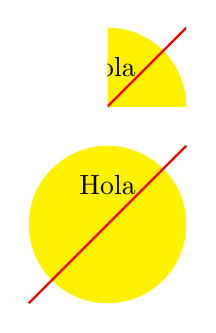
\begin{tikzpicture}
% Tambien podemos usar "clipping" para recortar. Eso si, hay que usarlo dentro de un entorno "scope" para evitar recortar todo el dibujo.
\begin{scope}
% Mostramos solo lo que este dentro de esta region que definimos con "clip".
\clip (0,0) rectangle (1,1);
\fill[yellow] (0,0) circle (1cm);

% Funciona con todo lo que pongamos, no solo fill
\draw[red, thick] (-1,-1) -- (1, 1);
\node at (0, 0.5) {Hola};
\end{scope}

% Vemos que pasa si ponemos lo mismo sin clipping.
\begin{scope}[yshift=-1.5cm] % Ventajas de scope: podemos mover una parte del dibujo con xshift/yshift. Tambien podriamos usar scale = 2 para doblarle el tamano, por ejemplo.
\fill[yellow] (0,0) circle (1cm);
\draw[red, thick] (-1,-1) -- (1, 1);
\node at (0, 0.5) {Hola};
\end{scope}
\end{tikzpicture}
\end{LTXexample}

\begin{LTXexample}[width=0.4\textwidth, pos=r]
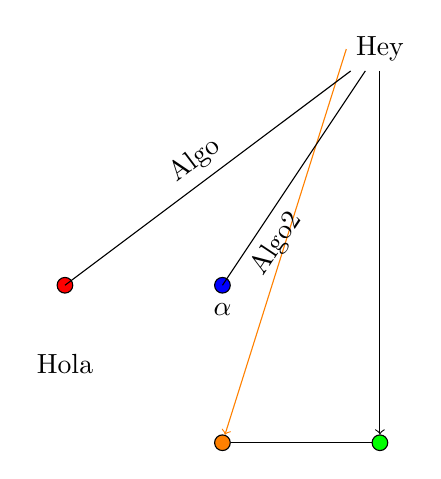
\begin{tikzpicture}
% Podemos poner nodos con texto o sin texto. Las llaves del final son necesarias siempre.
\node at (0, 1) {Hola};
\node[draw, circle, inner sep = 2pt, fill = red] at (0,2) {};

% Tambien se pueden poner etiquetas
\node[draw, circle, inner sep = 2pt, fill = blue, label = below:{$\alpha$}] at (2,2) {};

% Los nodos pueden ir nombrados para referenciarlos luego
\node[draw, circle, inner sep = 2pt, fill = orange] (A) at (2,0) {};
\node[draw, circle, inner sep = 2pt, fill = green] (B) at (4,0) {};
\draw (A) -- (B);

% Podemos hacerlo igual con los nodos con texto
\node (C) at (4, 5) {Hey};
\draw[->] (C) -- (B);

% Podemos decidir de que parte del nodo (south, west, north, east) sale la flecha
\draw[orange, ->] (C.west) -- (A);

% Y tambien podemos poner nodos en lineas
\draw (0,2) -- node[midway, above, sloped] {Algo} (C);
\draw (2,2) -- node[near start, below, sloped] {Algo2} (C);
\end{tikzpicture}
\end{LTXexample}

\begin{LTXexample}[width=0.4\textwidth, pos=r]
\usetikzlibrary{calc} % Para hacer calculos de puntos

\begin{tikzpicture}
% Dibujamos tres vertices de un triangulo
\node[draw, circle, inner sep = 2pt, fill = red, label = below:{$A$}] (A) at (0,0) {};
\node[draw, circle, inner sep = 2pt, fill = orange, label = below:{$B$}] (B) at (2.5,0) {};
\node[draw, circle, inner sep = 2pt, fill = green, label = above:{$C$}] (C) at (2,3) {};

% Ahora podemos hacer calculos y dibujar nodos donde queramos.
% Por ejemplo, un nodo a medio camino entre A y B
\node[draw, inner sep = 2pt, fill = blue] at ($(A)!0.5!(B)$) {};

% O sacar la recta perpendicular a AC que pasa por B
\draw (A) -- (C);
\draw[thick, dashed] (B) -- ($(A)!(B)!(C)$);

% Podemos sumar coordenadas
\node[draw, circle, inner sep = 2pt, fill = yellow, label = left:{$B + C$}] at ($(B) + (C)$) {};
\end{tikzpicture}
\end{LTXexample}

\begin{LTXexample}[width=0.4\textwidth, pos=r]

\begin{tikzpicture}
% Con colores tambien podemos hacer cosas chulas. Podemos combinarlos para sacar cosas distintas:
\fill[red!50!yellow] (0,0) rectangle (1,1);

% O hacer degradados
\fill[left color = red, right color = yellow] (2,0) rectangle (3,1);

% Y transparencias
\node at (4.5, 0.5) {Hola};
\fill[left color = red, right color = yellow, opacity = 0.3] (4,0) rectangle (5,1);
\end{tikzpicture}
\end{LTXexample}

\index{pgfplots}
\begin{LTXexample}[width=0.4\textwidth, pos=r]
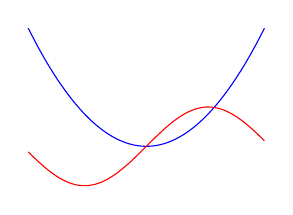
\begin{tikzpicture}
% Tambien podemos hacer funciones
\draw[scale=0.5,domain=-3:3,smooth,variable=\x,blue] plot ({\x},{\x*\x / 3});
\draw[scale=0.5,domain=-3:3,smooth,variable=\x,red] plot ({\x},{sin(\x r)});
% Nota: los senos y cosenos tikz los trata con grados. Hay que poner la r para que convierta a radiantes.
\end{tikzpicture}

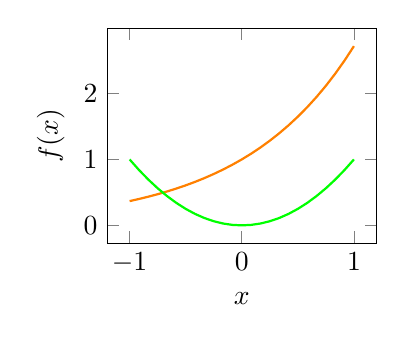
\begin{tikzpicture}
% Tambien se puede usar el entorno axis, que es mas facil de usar si solo queremos hacer graficas.
% Para activarlo, hay que poner \usepackage{pgfplots} en el preambulo.
\begin{axis}[width=5cm, domain = -1:1,	xlabel = $x$, ylabel = {$f(x)$}]
\addplot[color=orange, thick]{exp(x)};
\addplot[color=green, thick]{x^2};
\end{axis}
\end{tikzpicture}
\end{LTXexample}

\index{tikz-3dplot}
\index{3D}
\begin{LTXexample}[width=0.4\textwidth, pos=r]
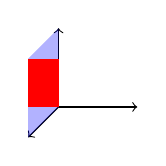
\begin{tikzpicture}
% Tikz tambien se maneja con coordenadas 3D
\draw[->] (0,0,0) -- (1,0,0);
\draw[->] (0,0,0) -- (0,1,0);
\draw[->] (0,0,0) -- (0,0,1);

% Aunque no del todo bien. Esto funciona
\fill[blue, opacity = 0.3] (0,0,0) -- (0,1,0) -- (0,1,1) -- (0,0,1) -- cycle;

% Pero esto no como queriamos
\fill[red] (0,0,0) rectangle (0,1,1);

% Para cosas en 3D mas avanzadas, ver
% tikz-3dplot
\end{tikzpicture}
\end{LTXexample}

\subsection{Un compilador más completo: latexmk}

\index{latexmk}
Al principio de este capítulo veíamos cómo funcionaba \LaTeX\ (\fref{sec:FuncionamientoLaTeX}), y que uno los problemas es que a veces hay que hacer varias pasadas para que funcione todo bien, lo cual puede ser un poco pesado. Por suerte, hay una solución llamada \textit{latexmk}, que es un compilador\footnote{En realidad es un script en Perl que llama a pdflatex y demás compiladores según convenga, pero para el caso es un compilador.} que se encarga de hacer todo esto de manera automática. Simplemente ejecutando \texttt{latexmk -pdf -silent documento.tex} compilará todo, haciendo tantas pasadas como haga falta.

La segunda ventaja de \textit{latexmk} es que nos permite compilar el documento de forma continua: cada vez que lo guardamos, \textit{latexmk} recoge los cambios y recompila para que nuestro lector de PDF pueda actualizar el documento\footnote{En Linux, Evince y Okular recargan el documento automáticamente. En OS X, Skim funciona muy bien.}. Para ello sólo tenemos que añadir el parámetro \textit{-pvc}: \texttt{latexmk -pdf -silent -pvc documento.tex}.

\textit{latexmk} tiene varias opciones más (ver su página de manual) y merece la pena probarlo y usarlo para quitarnos de problemas. Suele estar disponible como un paquete normal en las distribuciones Linux (\texttt{sudo apt-get install latexmk} funciona, por ejemplo) y también en MacPorts y Brew para OS X.

\subsection{Beamer: presentaciones con \LaTeX\ (o cómo dije adiós a Powerpoint)}

\index{Beamer}
Entre todas las cosas que permite hacer \LaTeX\, una de ellas es presentaciones con \textit{beamer}. Es una clase de documento que nos permitirá crear transparencias con toda la potencia de \LaTeX\ y olvidándonos de Powerpoint. Se escribe todo exactamente igual que en un docuemnto normal, salvo porque tenemos que agrupar el contenido en transparencias con \verb|\begin{frame}...\end{frame}|. No vamos a entrar mucho en detalle: simplemente pretendo dar una idea de que esto existe y es útil. Para una guía completa, \href{http://osl.ugr.es/CTAN/macros/latex/contrib/beamer/doc/beameruserguide.pdf}{la documentación de Beamer está muy bien}. También recomendaría echarle un ojo a los temas de Beamer para cambiar el estilo. \href{http://deic.uab.es/~iblanes/beamer_gallery/}{Aquí hay un directorio de los que vienen por defecto}, aunque yo personalmente prefiero \href{https://github.com/matze/mtheme}{mtheme}, que es bastante más ligero y con una tipografía bastante mejor.

\begin{minted}{latex}
\documentclass{beamer}

\usetheme{default} % O cualquier otro

\title{Adiós, Powerpoint}
\date{\today}
\author{Yo}

\begin{document}
  \maketitle

  \section{Sección}

  \begin{frame}{Título}
  \framesubtitle{Subtítulo}

    Hello, world!
  \end{frame}
\end{document}
\end{minted}

\section{Ampliando \LaTeX: Desarrollo de comandos, entornos, paquetes y clases}

Una de las ventajas de \LaTeX\ es que nos permite ``programar'' nuestros documentos, creando nuevos comandos y entornos y así automatizar todo lo posible nuestra escritura. Lo malo es que la sintaxis no es la más cómoda del mundo, y tiene bastantes cosas algo impredecibles. En cualquier caso, aquí vamos a ver una introducción sencilla a la programación de comandos y entornos en \LaTeX.

\subsection{Comandos y entornos}

A estas alturas ya deberíamos conocer más o menos cómo va \LaTeX\ (y si no, léase el comienzo de este capítulo): nosotros escribimos comandos y el procesador los va expandiendo con los argumentos que le pasamos. Sólo nos falta saber cómo definir un comando, y eso es bastante sencillo.


\cindex{newcommand}
\begin{minted}{latex}
% Definimos un nuevo comando
\newcommand{\micomando}{Contenido del comando}

% Si ahora escribimos esto:
\micomando
% En el documento aparecerá "Contenido del comando"

% Los comandos pueden recibir argumentos. Para ello, usamos la sintaxis
%   \newcommand{comando}[número de argumentos]{definición}
% En la definición, los #1, #2, ..., #n se sustituirán por el argumento
% en la posición correspondiente.
\newcommand{\yosoy}[1]{Hola, soy #1}

\yosoy{Guille} % -> "Hola, soy Guille"

% Los comandos pueden aceptar un único argumento opcional. Para ello,
% después del número de argumentos ponemos el valor que tendrá por defecto
% el argumento. El argumento opcional siempre es el primero.
\newcommand{\opcional}[2][]{Primero #1 y segundo #2}

\opcional{dos} % -> Primero y segundo dos
\opcional[uno]{dos} % -> Primero uno y segundo dos

% El argumento opcional puede tener un valor por defecto
\newcommand{\opcional}[2][tres]{Primero #1 y segundo #2}
\opcional{dos} % -> Primero tres y segundo dos
\end{minted}

De una forma bastante similar podemos definir los entornos, que son los que empiezan con \verb|\begin{...}| y acaban con \verb|\end{...}|.

\cindex{newenvironment}
\begin{minted}{latex}
% Sintaxis
\newenvironment{test}{esto se sustituye en el \begin{}}{esto se sustituye en el \end{}}

% Los argumentos siguen la misma sintaxis que para \newcommand.

% Ejemplo: un entorno con argumento opcional
\newenvironment{operacion}[1][]{\textsc{Operación #1}: }{\hline}

% Si ponemos esto
\begin{operacion}[prueba]
\[ 32 + 4 = 8\]
\end{operacion}

% Se sustituye después por:
\textsc{Operación prueba}: % La parte del \begin
\[ 32 + 4 = 8 \]
\hline % La parte del \end
\end{minted}

\cindex{renewcommand}
Si por lo que sea el comando o entorno que queremos definir ya está definido, simplemente tendremos que usar \texttt{renewcommand} o \texttt{renewenvironment}, con la misma sintaxis que antes.

\subsubsection{Manejo avanzado de argumentos}

Como se puede ver, la definición de nuevos comandos es bastante sencilla. Lo único malo es que la gestión de los argumentos es un poco tirando a mala: en cuanto queramos tener varios argumentos opcionales o tengamos muchos parámetros, la implementación de \LaTeX\ se nos va a quedar corta.

Para el primer problema, el paquete \index{xargs}\textit{xargs} da una solución: variantes \cindex{newcommandx}\texttt{newcommandx} y \cindex{newenvironmentx}\texttt{newenvironmentx}, que permiten definir múltiples argumentos opcionales. La sintaxis es muy sencilla y similar a la que acabamos de ver

\begin{minted}{latex}
% Sintaxis
\newcommandx{\comando}[nargs][1=valor por defecto arg1, ...]{definicion}

% Ejemplo:
\newcommandx{\convs}[3][1=,2=n,3=\infty]{\xrightarrow[#2\to #3]{#1}}

\convs % -> \xrightarrow{n \to \infty}{}
\convs[c.s.] % -> \xrightarrow{n \to \infty}{c.s.}
\convs[c.s.][x] % -> \xrightarrow{x \to \infty}{c.s.}
\convs[c.s.][x][0] % -> \xrightarrow{x \to 0}{c.s.}
\end{minted}

\index{pgfkeys}
El problema de tener muchos argumentos ya no se resuelve tan fácilmente. \href{http://tex.stackexchange.com/questions/34312/how-to-create-a-command-with-key-values}{Hay muchos paquetes} para poner argumentos en la forma \textit{clave = valor}. A mí personalmente me gusta \textit{pgfkeys}, así que pondré un ejemplo sencillo aquí:

\begin{minted}{latex}
% Primero se definen los argumentos
\pgfkeys{
	% Antes de nada, se agrupan en una "familia" las claves
	% y le decimos a pgf que entramos a definir esa familia
	/testkeys/.is family,
	/testkeys,

	% name será una clave, cuyo valor se guardará
	% en el comando \aname
	name/.store in = \aname,
	name/.value required,

	% Con .code podemos hacer que se ejecute un código
	% cuando nos pasan el argumento codearg. #1 se sustituye
	% por el valor correspondiente
	counter/.code = {\setcounter{test}{#1}},

	% Con .is choice podemos definir una serie de argumentos permitidos
	enum/.is choice,
	enum/true/.code = {\def\enumval{true}},
	enum/false/.code = {\def\enumval{false}}

	% Podemos definir un estilo "default" con valores por defect
	default/.style =
	  { name={empty}, enum=true, counter = 0}
}

% Ahora definimos el comando con un argumento opcional
\newcommand{\testcommand}[1][]{
	% Ejecutamos las claves opcionales, pasando primero "default"
	% para que, si #1 está vacío, se ejecuten las opciones por defecto
	\pgfkeys{/testkeys, default, #1}

	% Ahora podemos usar los comandos que hemos definido antes:
	El nombre es \aname, enum es \enumval y parece ser que tenemos
	un contador que vale \arabic{test}.
}

% Ejemplo:
\testcommand[name = test, counter = 2, enum = false]
	% -> El nombre es test, enum es false y parece ser que tenemos
	% un contador que vale 2

\testcommand
	% -> El nombre es empty, enum es true y parece ser que tenemos
	% un contador que vale 0
\end{minted}

\subsubsection{Comandos de bajo nivel \TeX\ y expansión de argumentos}

Justo en el ejemplo anterior, he puesto un comando que no hemos comentado: \verb|\def|. Lo he puesto más que nada como excusa para escribir esta sección. Ya voy avisando que nos estamos adentrando en cosas algo más técnicas de \LaTeX / \TeX\ y yo no tengo del todo lo claro lo que escribo aquí.

\cindex{def}
\verb|\def| es simplemente la forma de definir comandos en \TeX. Por decirlo de alguna forma, es un manejo a más bajo nivel que \LaTeX. En general, es recomendable usar \verb|\newcommand| porque es más robusto, hace algunas comprobaciones necesarias (como por ejemplo, que no estés redefiniendo un comando que ya existe) y es más fácil de usar. La ventaja que tiene \verb|\def| es que es más corto y para definir comandos sencillos, como en el ejemplo de arriba un \verb|\def\enumval{true}| es más cómodo.

\cindex{let}
Junto con \verb|\def|, me gustaría comentar el comando \verb|\let|, que también es bastante útil: nos permite darle un nombre alternativo a un comando. Digo que es especialmente útil porque con él podremos poner ``capas'' por encima de otros comandos ya existentes. Por ejemplo, supongamos que queremos redefinir el comando \verb|\section| para que, además de poner la sección, nos meta el título en el glosario con \verb|\index|. Tenemos que redefinir \verb|\section| pero no podemos eliminarlo del todo. Entonces haríamos algo así:

\begin{minted}{latex}
\let\oldsection\section % \oldsection tiene ahora el código de \section

% Así que ya podemos redefinir \section
\renewcommand{\section}[1]{
	\index{#1} % Hacemos lo que queremos nosotros antes
	\oldsection{#1} % Y ahora llamamos al comando \section de antes
}
\end{minted}

\cindex{newif}
Otra primitiva interesante de \TeX\ son las variables booleanas. Lo explico mejor con un ejemplo. Supongamos que queremos saber cuándo estamos en el apéndice del documento para que un comando cambie la salida. Entonces podríamos hacer algo así:

\begin{minted}{latex}
% En el preámbulo
\newif\if@inappendix
\@inappendixfalse % Por defecto estamos fuera del apéndice

\let\oldappendix\appendix % Nos guardamos \appendix
\renewcommand{\appendix}{ % Y lo redefinimos
	\@inappendixtrue % Cambiamos la variable a true
	\oldappendix % Y llamamos al comando \appendix viejo
}


% Ahora definimos el comando que sabe cuándo está en el apéndice
\newcommand{\mycommand}{
	\if@inappendix
		Estamos en el apéndice
	\else
		No estamos en el apéndice
	\fi
}
\end{minted}

Y ya que estamos, voy a mencionar un tema peliagudo, que es el de expansión de argumentos y comandos. Como decíamos al principio de este capítulo, \LaTeX\ funciona expandiendo argumentos y sustituyendo cosas: primero expande el comando y luego sus argumentos, así todo en orden. A veces, eso puede llevarnos a fallos, y querremos que se expandan primero los argumentos y después el comando, o también cambiar el orden de expansión de formas un poco extrañas.

Aquí es donde entran \verb|\expandafter|, \verb|\noexpand| y amigos similares, que controlan si el siguiente comando se expande o no. \href{http://tex.stackexchange.com/a/519/69094}{Esta respuesta de TeX.SX} explica más o menos bien cómo funcionan. Lo menciono aquí porque es importante saber que estas cosas existen, aunque personalmente todavía no he pasado del momento de programación aleatoria pegando \verb|\expandafter| y \verb|\noexpand| hasta que el comando funciona.

\subsection{Paquetes y clases}

Para poder reutilizar el código fácilmente, \LaTeX\ permite crear paquetes y clases de documentos. A grandes rasgos, no son más que archivos con comandos que se pegan ``a pelo'' en el documento en el que se incluyen. En ambos casos, eso sí, empiezan con una cabecera especial:

\begin{minted}{latex}
% Para clases (archivos .cls)
\NeedsTeXFormat{LaTeX2e}
\ProvidesClass{nombreclase}[YYYY/MM/DD Descripción]

% Para paquetes (archivos .sty)
\NeedsTeXFormat{LaTeX2e}
\ProvidesPackage{nombrepaquete}[YYYY/MM/DD Descripción]
\end{minted}

Cuando en un documento se incluye una clase con \verb|\documentclass| o un paquete con \verb|\usepackage|, el compilador de \LaTeX\ busca los correspondientes archivos \textit{.cls} y \textit{.sty} en los directorios de la instalación (a estos directorios mueve el script \textit{install} que tenemos en el repositorio las clases y paquetes que hemos creado), y también en el directorio donde está el documento \textit{.tex} que estemos compilando.

Para más detalles sobre cómo escribir paquetes y clases de documentos, es muy recomendable leerse \href{https://latex-project.org/guides/clsguide.pdf}{\LaTeXe\ for class and package writers}.

\subsection{Paquetes auxiliares para el desarrollo}

Ya para acabar con este tema, pongo aquí una pequeña referencia de paquetes que son bastante útiles a la hora de desarrollar comandos. Recuerdo que se puede ver la documentación de cada uno de ellos en Internet o, desde la consola de comandos de tu sistema, con \textit{texdoc nombrepaquete}.

\begin{itemize}
\item \textit{etoolbox}: Varias herramientas que vienen bien para el desarrollo. Especialmente útiles los \textit{hooks} o ganchos para poner código al final o al principio del documento y otros entornos.
\item \textit{ifthen}: Como su nombre indica, permite escribir fácilmente sentencias \textit{if-then-else}.
\item \textit{mfirstuc}: Da un cmando para poner el primer carácter de una palabra en mayúsculas.
\item \textit{xspace}: Provee el comando \verb|\xspace|, para poner espaciado correcto detrás de comandos matemáticos, evitando poner espacios de más o de menos cuando definimos algo.
\item \textit{xstring}: Permite trabajar con cadenas, manipulándolas, comparándolas, etc.
\end{itemize}
